%\section{対象計算領域の設定} \label{sec:domain}
\section{\SecBasicDomainSetting} \label{sec:domain}
%=======================================================================

%\Item{\SubsecRelationOfResoGridProcess}
各設定を行う前に、\scalerm での対象計算領域の格子点数とMPIプロセスの関係を整理しておく。
計算領域は、水平格子間隔と格子点数を指定することで決定されるようになっている。
図\ref{fig:domain}は、
計算領域、水平格子間隔、格子数、及びMPIプロセス数の関係を示している。
水平方向に2次元の領域分割を行うことで並列化がなされている。

これらは、\namelist{PARAM_INDEX}内の\nmitem{IMAX,JMAX}、
\namelist{PARAM_PRC}内の\nmitem{PRC_NUM_X,PRC_NUM_Y}で設定する。
%水平格子間隔については、\namelist{PARAM_GRID}内の\nmitem{DX,DY}で設定する。

ここで、注意すべきことは、「指定する格子点数は各プロセスが受け持つ値」であることである。
設定する格子数(\nmitem{IMAX, JMAX,KMAX})は、
1つのMPIプロセスが担当する格子点数を与える仕様となっている。
すなわち、計算領域は、
水平格子間隔、格子点数とともに各方向のMPIプロセス数を考慮して決定する必要がある。

図\ref{fig:domain}に示すように、
MPIプロセス数が$n$(=\verb|PRC_NUM_X|$\times$\verb|PRC_NUM_Y|)の時、
計算領域は、\XDIR に\nmitem{PRC_NUM_X}個、\YDIR に\nmitem{PRC_NUM_Y}個に分割される。
以上の関係から、計算領域全体のそれぞれの方向の格子点数および総格子点数は、
\begin{eqnarray}
&& 領域内{\XDIR} の格子数 = \left(\verb|IMAX| \times \verb|PRC_NUM_X|\right)
   \times (\verb|KMAX| )  \label{eq:xgridnum}\\
&& 領域内{\YDIR}の格子数 = \left(\verb|JMAX| \times \verb|PRC_NUM_Y|
   \times (\verb|KMAX|\right)  \label{eq:ygridnum}\\
&& 領域内の総格子数 = \left(\verb|IMAX| \times \verb|PRC_NUM_X|\right)
   \times (\verb|JMAX| \times \verb|PRC_NUM_Y|)
   \times (\verb|KMAX| )  \nonumber
\end{eqnarray}
の関係となる。
ここで、\nmitem{KMAX}は、鉛直方向の格子点数であり、
\namelist{PARAM_INDEX}内の項目で指定されている。
次節以降では、MPIプロセス数、格子数、格子間隔、
それぞれの設定方法について詳しく説明する。

\begin{figure}[h]
\begin{center}
  \includegraphics[width=0.8\hsize]{./figure/domain_decomposition.eps}\\
  \caption{計算領域に対する、水平格子間隔(DX, DY)、1MPIプロセスあたりの格子数(IMAX, JMAX)、MPIプロセス数(PRC\_NUM\_X, PRC\_NUM\_Y)の関係。
水色領域は、ある1つのMPIプロセスが担当する領域。}
  \label{fig:domain}
\end{center}
\end{figure}

\subsection{\SubsecDomainSetting} \label{subsec:relation_dom_reso2}

前節で述べた関係が理解できれば、領域の設定は容易である。
すなわち、式(\ref{eq:xgridnum},\ref{eq:ygridnum})を使って、
\begin{eqnarray}
&& {\XDIR} の領域の長さ = {\XDIR} の格子点数 \times \verb|DX| \nonumber\\
&& {\YDIR}の領域の長さ = {\YDIR}の格子点数 \times \verb|DY| \nonumber
\end{eqnarray}
となる。ここで、\nmitem{DX,DY}は、後述するように
\namelist{PRAM_GRID}で指定されるものである。
逆算して、解像度と領域の大きさをを決めて、MPIプロセス数が決まると、
ローカルな領域の格子点数が決まる。

\subsection{\SubsecMPIProcess} \label{subsec:relation_dom_reso3}

MPIプロセス数は、設定ファイルの\namelist{PARAM_PRC}で指定する。
\scalerm の入出力ファイルは、MPIプロセス毎に分割されているため、
MPIプロセス数を変更すると分割ファイル数も必ず変わることになる。
従って、例えば、2-MPI並列用に作成した初期値ファイルは、
4-MPI並列のモデル実行には使用できない。
MPIプロセス数を変更するには、
\verb|pp_***.conf|、\verb|init_***.conf|、\verb|run_***.conf| の
すべてを編集・変更し、\verb|pp|, \verb|init| から行う必要がある。\\

\noindent {\small {\gt
\ovalbox{
\begin{tabularx}{140mm}{lX}
\verb|&PARAM_PRC| & \\
\verb| PRC_NUM_X       = 2,| & ; {\XDIR}(東西方向)のMPI並列分割数 \\
\verb| PRC_NUM_Y       = 1,| & ; {\YDIR}(南北方向)のMPI並列分割数 \\
\verb|/|\\
\end{tabularx}
}}}\\


全MPIプロセス数は、\verb|PRC_NUM_X| $\times$ \verb|PRC_NUM_Y|  となり、
上記の例では、\XDIR に2分割、\YDIR に1分割(分割なし)の
2-MPI並列ということになる。

実行時にMPIコマンドに指定するMPIプロセス数は、
この総MPIプロセス数を指定しなければならない。
この条件を満たさない場合は、下記のメッセージが
LOGファイルなどに出力されて計算は行われず、直ちに終了する。

\noindent {\small {\gt
\ovalbox{
\begin{tabularx}{140mm}{l}
\verb|xxx total number of node does not match that requested. Check!| \\
\end{tabularx}
}}}\\





\subsection{\SubsecGridNumSettng} \label{subsec:relation_dom_reso4}
%-----------------------------------------------------------------------

格子数の設定は、設定ファイル(\verb|***.conf|)の\namelist{PARAM_INDEX}で行う。
以下で設定する水平格子数の値は、1つのMPIプロセス当たりの値であることに注意が必要である。\\

\noindent {\small {\gt
\ovalbox{
\begin{tabularx}{140mm}{lX}
\verb|&PARAM_INDEX| & \\
\verb| KMAX = 97,|  & 鉛直層数 \\
\verb| IMAX = 20,|  & プロセスあたりの{\XDIR} の格子点数 \\
\verb| JMAX = 25,|  & プロセスあたりの{\YDIR}の格子点数 \\
\verb|/|\\
\end{tabularx}
}}}\\



\subsection{\SubsecGridIntvSettng} \label{subsec:gridinterv}
%-----------------------------------------------------------------------
\scalerm では、水平方向に格子間隔を一定値で設定する。
鉛直方向には、均等間隔でも任意の格子点位置を直接指定することもできる。
以下で説明する
\textcolor{red}{\bf 格子間隔の設定は、pp\_***.conf、init\_***.conf、run\_***.confの
設定ファイルの間で一致させなければならないことに注意が必要である。}

~\\

%-----------------------------------------------------------------------&
第\ref{subsec:buffer}節で述べる緩和領域を覗き、
水平格子間隔は等間隔でしか設定できない。
鉛直格子間隔については、任意に定義することが可能である。
すべての方向について等間隔で設定する場合には、以下のように
設定ファイルの\namelist{PARAM_GRID}の\nmitem{DX,DY,DZ}に
それぞれ、東西、南北、鉛直方向の格子間隔を指定する。
単位はmである。

\noindent {\small {\gt
\ovalbox{
\begin{tabularx}{140mm}{lX}
\verb|&PARAM_GRID  | & \\
\verb| DX = 500.D0,| & ; {\XDIR}(東西方向)の格子間隔\\
\verb| DY = 500.D0,| & ; {\YDIR}(南北方向)の格子間隔\\
\verb| DZ = 500.D0,| & ; {\ZDIR}(鉛直方向)の格子間隔\\
\verb|/|\\
\end{tabularx}
}}}\\


以下に、鉛直方向での任意の格子点位置を指定する場合の設定を示す。
鉛直方向は、ローレンツ格子を採用しており、
速度成分定義格子点とスカラー定義格子点が半格子分ずれた食い違い格子にになっている。
ここでは、スカラー量を定義している格子点をセンターポイントと呼び、
半格子ズレた格子点をフェイスポイントと呼ぶ(図\ref{fig:scale_grid}参照)。

直接格子点の位置を指定する場合は、フェイスポイントの位置を
\namelist{PARAM_GRID}の中の\nmitem{FZ(:)}で配列として与えればよい。
\footnote{指定の際には、シミュレーションの計算精度
(モデルのコンパイル時に指定した浮動小数点の精度。デフォルトでは倍精度)を用いることが望ましい。}
また、\nmitem{FZ(:)}で指定する値の数は、鉛直層数
(\namelist{PARAM_INDEX}の\nmitem{KMAX})と一致させる必要がある。
例として理想実験のチュートリアルのrun.confファイル
( run\_R20kmDX500m.conf )を下記に示す。

\noindent {\small {\gt
\ovalbox{
\begin{tabularx}{140mm}{lX}
\verb|&PARAM_GRID|     & \\
\verb| DX = 500.D0,|   & {\XDIR} の格子間隔(等間隔)[m]\\
\verb| DY = 500.D0,|   & {\YDIR}の格子間隔(等間隔)[m]\\
\verb| FZ(:) = |       & {\ZDIR}のフェイスポイントの位置[m] \\
\verb|    80.000000000000000      ,| & \\
\verb|    168.00000190734863      ,| & \\
\verb|    264.80000610351567      ,| & \\
\verb|     〜 中略 〜|           & \\
\verb|    14910.428862936289      ,| & \\
\verb|    15517.262523292475      ,| & \\
\verb|    16215.121232702089      ,| & \\
\verb|    17017.658748523147      ,| & \\
\verb|    17940.576891717363      ,| & \\
\verb|    19001.932756390710      ,| & \\
\verb|    20222.492000765058      ,| & \\
\verb| BUFFER_DZ = 5000.D0,|          & 第\ref{subsec:buffer}節参照\\
\verb| BUFFFACT  =   1.0D0,|          & 第\ref{subsec:buffer}節参照\\
\verb|/|\\
\end{tabularx}
}}}\\


\begin{figure}[tb]
\begin{center}
  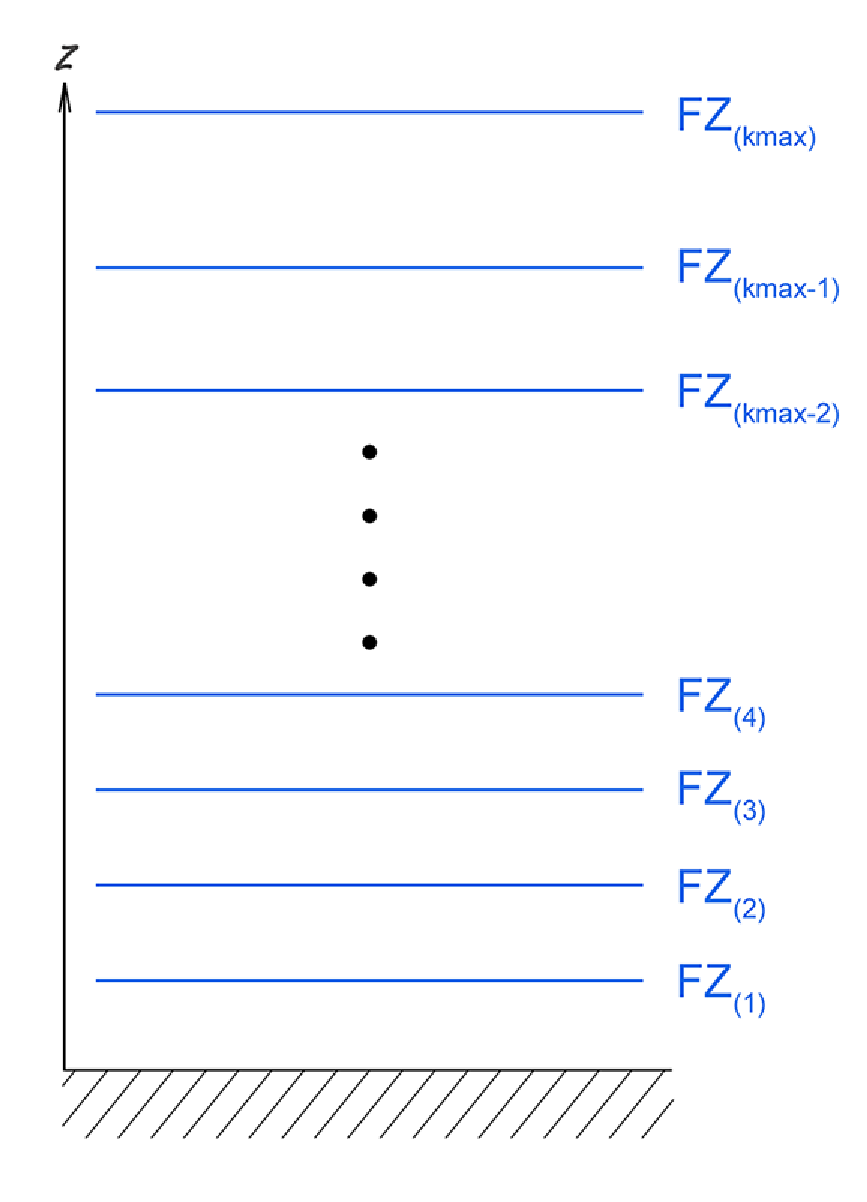
\includegraphics[width=0.4\hsize]{./figure/verticalface.eps}\\
  \caption{\scalerm の鉛直格子の定義点。\namelist{PARAM_GRID}で\nmitem{FZ}を指定する時は、ハロを除いた計算領域下端の格子から$k=1$として与える。}
  \label{fig:scale_grid}
\end{center}
\end{figure}
なお、これらの指定では、
標高0mでの格子点として設定され、標高を持つ位置では山岳に沿った座標系によって適切に処理される。


格子点位置は任意に設定できるが、場合によっては計算不安定につながる。
鉛直層の設定については、作成をサポートするツールが、\texttt{scale-\version/scale-rm/util/makevgrid/}
ディレクトリの中に`make\_vgrid.f90''というFortranプログラムと
いくつかのサンプルnamelistが用意されているので、参考にされたい。
ツールをコンパイルして実行すれば直ちに設定ファイルに貼り付けて使用できる
\nmitem{FZ(:)}の値が作成される。

\subsection{\SecAdvanceMapprojectionSetting} \label{subsec:adv_mapproj}
%------------------------------------------------------
\scalerm では、まず実距離に基づいた格子点が配置され、その格子点位置と緯度経度基準点の情報を元に、
それぞれの投影法を用いた際の各格子点での緯度・経度座標が計算される。
緯度・経度情報は、すべてのSCALEのNetCDF形式の出力ファイルに含まれている。\\
計算領域の位置と投影法は、設定ファイルの\nmitem{PARAM_MAPPROJ}の項目を編集することで設定できる。
\textcolor{red}{\bf この設定も、pp\_***.conf、init\_***.conf、run\_***.confの設定ファイルの間で
必ず一致させなければならない。}はじめに下記の例をもとに説明する。\\

\noindent {\small {\gt
\ovalbox{
\begin{tabularx}{140mm}{l}
\verb|&PARAM_MAPPROJ| \\
\verb| MPRJ_basepoint_lon = 138.727778D0,| \\
\verb| MPRJ_basepoint_lat = 35.360556D0,| \\
\verb| MPRJ_type          = 'MER',| \\
\verb|/| \\
\end{tabularx}
}}}\\

\begin{table}[b]
\begin{center}
\caption{SCALEで選択できる地図投影法}
\begin{tabularx}{150mm}{|l|X|} \hline
 \rowcolor[gray]{0.9} \verb|MPRJ_type| & 地図投影法 \\ \hline
 \verb|NONE| & 地図投影なし(理想実験用)、デフォルト \\ \hline
 \verb|LC|   & ランベルト正角円錐図法              \\ \hline
 \verb|PS|   & ポーラーステレオ図法                \\ \hline
 \verb|MER|  & メルカトル図法                     \\ \hline
 \verb|EC|   & 正距円筒図法                       \\ \hline
\end{tabularx}
\label{tab:map_proj}
\end{center}
\end{table}

\noindent
まず\nmitem{MPRJ_basepoint_lat}と\nmitem{MPRJ_basepoint_lon}は、
計算領域の中心の緯度・経度を表す。
SCALE-RMでは、北緯を正、南緯を負の値として表現し、
経度は0度を起点に右回りで表現するため、
この設定例では計算領域の
中心が北緯35.360556度、東経138.727778度に位置することになる。
この場所を中心に指定された大きさで、計算領域が設定される。\\
\nmitem{MPRJ_type}は、地図投影法の種類を表しており、\verb|MER|はメルカトル図法を意味する。
\scalerm で現在選択できる地図投影法とその指定文字列は表\ref{tab:map_proj}のとおりである。
メルカトル図法を用いた場合、投射する円筒に接する基準緯線は\nmitem{MPRJ_M_lat}で任意の値に設定する。
通常、基準緯線は赤道にとることが多いが、基準緯線に近いほど歪みが少なく正確に記述できるので、
\nmitem{MPRJ_M_lat}を指定しない場合は\nmitem{MPRJ_basepoint_lat}が基準緯線として用いられる。

\proofcomment{\nmitem{MPRJ_basepoint_lat}と\nmitem{MPRJ_M_lat}の使い分けの説明が不足しています。
記述してください.(八代)しました。}

投影法の中でも利用頻度が高いランベルト正角円錐図法の設定について以下に説明する。
ここでは、現実大気実験チュートリアルで使用した\verb|run.conf|ファイルを例に挙げる。\\

{\small {\gt
\ovalbox{
\begin{tabularx}{140mm}{l}
\verb|&PARAM_MAPPROJ| \\
\verb| MPRJ_basepoint_lon = 135.220404D0,| \\
\verb| MPRJ_basepoint_lat = 34.653396D0,| \\
\verb| MPRJ_type          = 'LC',| \\
\verb| MPRJ_LC_lat1       =  30.00D0,| \\
\verb| MPRJ_LC_lat2       =  40.00D0,| \\
\verb|/| \\
\end{tabularx}
}}}\\

\noindent
\scalerm では、2標準緯線型の投影方法を採用している。
両標準緯線に挟まれた領域では、
緯線・経線の長さの比が地球楕円体面上における長さの比と近くなるように調節される。
南側、北側の標準緯線はそれぞれ\nmitem{MPRJ_LC_lat1}と\nmitem{MPRJ_LC_lat2}で設定する。
値の単位はdegreeである。

さらに下記のように\nmitem{MPRJ_basepoint_x}と\nmitem{MPRJ_basepoint_y}という変数を用いることで、
地図投影中心と計算領域中心をずらすことができる。\\~\\

{\small {\gt
\ovalbox{
\begin{tabularx}{140mm}{l}
\verb|&PARAM_MAPPROJ| \\
\verb| MPRJ_basepoint_lon = 135.220404D0,| \\
\verb| MPRJ_basepoint_lat = 34.653396D0,| \\
\verb| MPRJ_basepoint_x   = 100.0D0,| \\
\verb| MPRJ_basepoint_y   = 100.0D0,| \\
\verb| MPRJ_type          = 'LC',| \\
\verb| MPRJ_LC_lat1       =  30.00D0,| \\
\verb| MPRJ_LC_lat2       =  40.00D0,| \\
\verb|/| \\
\end{tabularx}
}}}\\~\\

\noindent
\nmitem{MPRJ_basepoint_x}と\nmitem{MPRJ_basepoint_y}は、地図投影中心の位置を、
計算領域の南西端(左下角)からの距離で指定するパラメータで、単位はメートルである。
これらを指定しない場合、地図投影中心は計算領域中心に設定される。
地図投影中心を指定しない場合とした場合を比較したものを図\ref{fig:map_lc}に示す。
図\ref{fig:map_lc}aは、デフォルト設定で地図投影中心と計算領域中心が一致している場合、
図\ref{fig:map_lc}bは、地図投影中心をずらすよう指定した場合の関係を表している。
図\ref{fig:map_lc}bでは計算領域の南西端から
\nmitem{MPRJ_basepoint_x}と\nmitem{MPRJ_basepoint_y}で指定した距離だけ離れた位置に投影中心が設定される。

\begin{figure}[t]
\begin{center}
  \includegraphics[width=0.8\hsize]{./figure/LC_latlon_xy.eps}\\
  \caption{投影中心と計算領域の関係:(a)はデフォルト設定の場合、(b)は投影中心の位置を計算領域中心からずらした場合。
  赤線の矩形が計算領域を表す。}
  \label{fig:map_lc}
\end{center}
\end{figure}

\subsection{\SecBasicBufferSetting} \label{subsec:buffer}
%-----------------------------------------------------------------------
モデル最上層では意図しない重力波の反射が起こる。
また、側面境界では現実大気実験を行う際に境界条件と対象領域の間に値の不一致が起こる。
これを回避するため、「緩和領域」を設ける。
\scalerm では計算領域の境界のすぐ内側に緩和領域を設定することができる。
緩和領域の格子では、指定された値(境界値データ、親領域のデータなど)に対して
ある時定数で緩和される。以下これをナッジングと呼ぶ(上層における緩和はレイリーダンピングと呼ばれることが多い)。
緩和領域の幅は、設定ファイルの\namelist{PARAM_GRID}の中で設定する。
以下に例を示す。
設定はすべての設定ファイルにおいて共通していなければならない。\\

\noindent {\small {\gt
\ovalbox{
\begin{tabularx}{150mm}{lX}
\verb|&PARAM_GRID  |            & \\
 \verb|BUFFER_DZ = 5000.D0,   | & ; {\ZDIR}(モデルトップから下向き方向)の緩和領域の幅 [m]\\
 \verb|BUFFER_DX = 300000.D0, | & ; {\XDIR} (東西方向)の緩和領域の幅 [m]\\
 \verb|BUFFER_DY = 300000.D0, | & ; {\YDIR}(南北方向)の緩和領域の幅 [m]\\
 \verb|BUFFFACT  = 1.D0,      | & ; 緩和領域内の格子間隔に対するストレッチ係数(デフォルトは1.0)\\
\verb|/|\\
\end{tabularx}
}}}\\

水平方向には東西南北の四方境界に緩和領域が設定されるが、
鉛直方向には計算領域の上端にのみ緩和領域が設定され、下端には設定されない。
%
緩和領域は、計算領域内に設定されるため、
ナッジングの影響を受けない領域(緩和領域を除いた範囲)は
計算領域よりも狭くなることに注意が必要である。

\subsubsection{緩和領域の格子間隔をストレッチさせる}

緩和領域の格子間隔は、基本的に
\namelist{PARAM_GRID}の中の\nmitem{DX, DY, DZ}で指定した通りであるが、
\nmitem{BUFFFACT}に1以上の値を設定することで、ストレッチさせることも可能である。
ただし、格子間隔を等間隔で指定した場合、
この\nmitem{BUFFFACT}の設定は、X, Y, {\ZDIR}すべてに適用される。
それぞれの方向に別々に設定したい場合は、\nmitem{BUFFFACT_X}, \nmitem{BUFFFACT_Y}, \nmitem{BUFFFACT_Z}を指定する。
{\ZDIR}の層レベルを任意の格子点位置に指定する場合、
すなわち、\nmitem{FZ(:)}を与える場合(第\ref{subsec:gridinterv}節参照のこと)にはストレッチの設定は適用されない。

緩和領域内の格子間隔 (\verb|BDX|) は次の通り決定される。
\begin{eqnarray}
 \verb|BDX(|n\verb|)| &=& \verb|DX| \times \verb|BUFFFACT|^n \nonumber
\end{eqnarray}
ここで、$n$は緩和領域内の格子点番号を表し、計算領域の内側から外側へ向かって番号が振られる。
緩和領域の格子間隔は、
\nmitem{BUFFFACT=1.0}ならば内部領域と同じであり、
\nmitem{BUFFFACT=1.2}ならば内側から外側(境界)に向かって1.2倍の割合で広がっていく。
\nmitem{BUFFFACT}はいくつに設定しても良いが、計算の安定性を考慮すると 1.0から1.2 が推奨である。

緩和領域の格子数 \verb|ibuff|は、
\begin{eqnarray}
\sum_{n=1}^{\verb|ibuff|} \verb|BDX|(n) \ge \nmitemeq{BUFFER_DX} \nonumber
\end{eqnarray}
の関係を満たす最小の整数で自動的に計算され、緩和領域の大きさ\verb|BUFFER|$_x$は、
\[
  \verb|BUFFER|_x = \nmitemeq{DX} \times \frac{ \nmitemeq{BUFFFACT}^{\texttt{\detokenize{ibuff}}-1 }}{ \nmitemeq{BUFFFACT}-1 }
\]
となる。
結局、緩和領域を除いた計算領域の大きさは、
\[
\nmitemeq{DX} \times ( \nmitemeq{IMAX} \times \nmitemeq{PRC_NUM_X} - 2 \times \verb|ibuff| )
\]
となる。
%
緩和領域の幅\nmitem{BUFFER_DX}が同じでも、
\nmitem{BUFFFACT}の値を大きくすると緩和領域に用意される格子数は少なくなる。
ここでは、{\XDIR} の説明をしたが、{\YDIR}、{\ZDIR}も同様である。
ただし、{\ZDIR} については下端には緩和領域が取られないため、緩和領域を除いた計算領域の大きさは
\[
\nmitemeq{DZ} \times ( \nmitemeq{KMAX} - \verb|kbuff| )
\]
となる。

\proofcomment{ここは何度よんでも理解がしにくいです。結局この設定によって、真の対象領域は、
  どこなのか?を図に書いて説明してください}
\replycomment{式を追加しました。図はヨッシーに発注しています。(西澤)}
\proofcomment{了解しました。絵の追加を待って、本件終了させます。(富田)}
\replycomment{図を追加しました(吉田)}


一般に、緩和領域の大きさ、緩和格子点の数については、解く問題により、明確な指標はない。
\scalerm では、鉛直方向(計算領域トップ)の緩和格子点は5点以上、
水平方向(側面境界付近)の緩和格子点は20〜40点程度を推奨している。
実験設定や事例によっては、さらに緩和格子点を増やしたり、
ストレッチ係数を用いて緩和領域を広げたり、
緩和の時定数を調整したりする必要があるだろう。
時定数とは、目標値との差が$1/e$になるまでの時間である。
緩和の時定数は、
\namelist{PARAM_ATMOS_BOUNDARY}の中の
\nmitem{ATMOS_BOUNDARY_taux,ATMOS_BOUNDARY_tauy,ATMOS_BOUNDARY_tauz}によって秒単位で設定する。
デフォルトの値は $10 \Delta t$ であり、これは、10タイムステップで$1/e$になることに相当する。
タイムステップについては、第\ref{sec:timeintiv}節を参照のこと。

\begin{figure}[t]
\begin{center}
  \includegraphics[width=0.8\hsize]{./figure/buffer_xz.eps}\\
  \caption{計算領域における緩和領域の配置:斜線部分が緩和領域を意味する。
  図はXZ断面だが、Y方向にも同一の配置である。}
  \label{fig:buff_xz}
\end{center}
\end{figure}


\subsection{\SecBasicTopoSetting} \label{subsec:basic_usel_topo}
%-----------------------------------------------------------------------

\scalerm では地形データに対しモデル下端の格子面を傾斜させて地形を表現する山岳に沿った座標系を採用している。
水平の最大格子間隔を$DX_{max}$[m]、鉛直の最小格子間隔を$DZ_{min}$[m]とすると、許容される最大の地形傾斜角度$\theta_{max}$[deg]は次の式で計算される。

\[ \theta_{max} = \arctan( \mathrm{RATIO} \times \mathrm{DZ_{min}}/\mathrm{DX_{max}} ) \times 180/\pi \]

\scalerm ではRATIOのデフォルト値を1.0に設定している。
RATIOの設定を、1.0よりも大きくすれば地形がより細かく、1.0よりも小さくすれば地形がより粗く表現される。
ただしRATIOを1.0よりも大きくした場合、計算が途中で破綻する危険性が高くなる。

地形の設定は、設定ファイルの\namelist{PARAM_CNVTOPO}の中で設定する。
以下に例を示す。\\

\noindent {\small {\gt
\ovalbox{
\begin{tabularx}{150mm}{lX}
\verb|&PARAM_CNVTOPO  |                  & \\
 \verb|CNVTOPO_name                  = "GTOPO30", | & ; 使用する地形データ名\\
 \verb|CNVTOPO_smooth_maxslope_ratio = 1.0,       | & ; DZのDXに対する比の倍率 \\
 \verb|CNVTOPO_smooth_local          = .true.,    | & ; 最大傾斜角度を超えた格子のみ平滑化を行うかどうか \\
 \verb|CNVTOPO_copyparent            = .false.,   | & ; 緩和領域に親ドメインの地形をコピーするかどうか \\
\verb|/|\\
\end{tabularx}
}}}\\


使用する地形データの名称を与え、地形データを読み込む。
\scalerm ではGTOPO30、または国土地理院による高精度地形データ(DEM50M)をサポートしている。

最大傾斜角度を超える傾斜角が与えられた地形データ内に検出された場合、
それを最大傾斜角度以下になるように、反復計算を用いて徐々に平滑化を実行する。
このとき、最大傾斜角度を超えた格子のみ平滑化を行うか、計算領域全体で行うかを選択することができる。
前者は、最大傾斜角度以内のシャープな地形構造を残すことができるので、細かな地形表現を望む場合に選択する。

上記の計算式で分かるように、許容される最大傾斜角度は空間解像度に応じて変わる。
一般的に、多段ネスティング計算を行う場合、
子ドメインのほうが空間解像度が細かいため、地形もシャープに表現される。
このとき、親ドメインと子ドメインの地形表現が異なるために、
子ドメインの緩和領域に挿入される親ドメインの大気データを外挿する必要が発生し、不整合を起こすことがある。
これを回避するために、
\nmitem{CNVTOPO_copyparent}を\verb|.true.|とすることで、親ドメインの地形を子ドメインの緩和領域にコピーすることができる。
親ドメインが存在しない場合は\nmitem{CNVTOPO_copyparent}を必ず\verb|.false.|に設定しなければならない。
